\documentclass[DM,authoryear,toc]{lsstdoc}
% GENERATED FILE -- edit this in the Makefile
\newcommand{\lsstDocType}{DMTN}
\newcommand{\lsstDocNum}{296}
\newcommand{\vcsRevision}{3a0ea4e-dirty}
\newcommand{\vcsDate}{2024-08-23}


% Package imports go here.

% Local commands go here.

%If you want glossaries
%\input{aglossary.tex}
%\makeglossaries

\title{Calculations of Image and Catalog Depth}

% This can write metadata into the PDF.
% Update keywords and author information as necessary.
\hypersetup{
    pdftitle={Calculations of Image and Catalog Depth},
    pdfauthor={Alex Drlica-Wagner},
    pdfkeywords={}
}

% Optional subtitle
% \setDocSubtitle{A subtitle}

\author{%
Alex Drlica-Wagner,
Eric Neilsen,
Lynne Jones,
Peter Ferguson
}

\setDocRef{DMTN-296}
\setDocUpstreamLocation{\url{https://github.com/lsst-dm/dmtn-296}}

\date{\vcsDate}

% Optional: name of the document's curator
% \setDocCurator{The Curator of this Document}

\setDocAbstract{%
We describe several avenues toward assessing the depth of LSST observations using source catalogs and exposure summary statistics. We validate these estimates against each other, and against predicted depth estimates from the LSST Operations Simulator.
}

% Change history defined here.
% Order: oldest first.
% Fields: VERSION, DATE, DESCRIPTION, OWNER NAME.
% See LPM-51 for version number policy.
\setDocChangeRecord{%
  \addtohist{2}{2024-11-29}{Addressing review comments.}{Alex Drlica-Wagner}
  \addtohist{1}{2024-10-16}{First complete draft.}{Alex Drlica-Wagner}
}
\setDocDate{2024-11-29}

\begin{document}

% Create the title page.
\maketitle
% Frequently for a technote we do not want a title page  uncomment this to remove the title page and changelog.
% use \mkshorttitle to remove the extra pages

% ADD CONTENT HERE
% You can also use the \input command to include several content files.

\section{Introduction}

The ``depth'' of a survey is colloquially used to describe the faintest astronomical object that can be detected and accurately measured. However, because astronomical objects cover a broad range of shapes and sizes, and surveys have variable performance along many avenues (angular resolution, sky brightness, instrumental noise, etc.), there is no unique definition for ``depth''. Thus, it is conventional to specify precise depth metrics that can be uniquely defined in terms of the properties of the survey. Although several metrics have been proposed and used by astronomical surveys \citep[e.g.,][]{Rykoff:2015, DES-DR2}, LSST has focused primarily on measurements of the limiting magnitude for unresolved point-like sources detected at a signal-to-noise ratio ($SNR$) of $5$. This metric is canonically referred to as  ``$m5$'' or in common speech as the ``5$\sigma$ limiting magnitude'' \citep[e.g.,][]{SMTN-002}. Of course, the depth can be calculated at an arbitrary SNR, although ${SNR} = 5$ ($m5$) and ${SNR} = 10$ ($m10$) are the most common values chosen.

Several documents have laid out the approach to calculating $m5$ in terms of the properties of the LSST system. In particular, \citet{LSE-40} provided a quantitative derivation of $m5$, which has been used to set the LSST System Requirements (LSR) \citep{LSE-29}. More recently, \citet{SMTN-002} provided a framework for predicting $m5$ given current LSST system throughputs and rapidly calculating $m5$ for the LSST Operations Simulator (OpSim). Here, we translate the established framework for calculating $m5$ into the LSST Science Pipelines in order to provide self-consistent estimates of $5\sigma$ limiting magnitude.\footnote{The code for the analyses described here can be found in \href{https://github.com/lsst-dm/vv-team-notebooks/tree/main/notebooks}{\texttt{DM-45573\_Depth\_Estimates.ipynb}}.} In particular, we estimate the depth in two different and complementary ways: (1) directly from the catalogs by selecting point-like sources that have measured ${SNR} \approx 5$, and (2) from summary statistics (i.e., seeing, sky brightness, transparency, read noise) that are calculated on a per-exposure basis. While these are different techniques for measuring the noise, they both share the same analytic calculation of the variance (i.e., the catalog flux uncertainties come from the variance plane, which is calculated from the same information as the exposure summary statistics). Inaccuracy in the analytic variance would thus be manifested in both estimates. A third complementary and more independent technique would be to measure the variance directly from repeated observations of faint (or sky) sources. This direct variance measurement is an important validation of the analytic variance calculation; however, it is subject to biases from the presence of sub-threshold sources \citep[e.g.,][]{Eckert:2020}. The direct estimation of the variance from repeat observations is left to future work.

\section{Depth Estimates Using Object Catalogs}

The most straightforward mechanism for estimating the 5$\sigma$ limiting magnitude, $m5$, comes from selecting sources with ${SNR} \approx 5$, where $SNR$ is defined as
\begin{equation}
\label{eqn:flux_snr}
SNR = \frac{f}{\sigma_f},
\end{equation}
where $f$ is the flux of the source and $\sigma_f$ is the flux uncertainty.
Estimating $SNR \approx 5$ can be done most directly with a simple cut (e.g., $4.75 < SNR < 5.25$), as implemented by the \href{https://github.com/lsst/analysis_tools/blob/1eab82deb581fff22c4bd353dabf200f98e2518d/python/lsst/analysis/tools/atools/limitingMagnitudeMetric.py}{\texttt{FiveSigmaPointSourceDepthMetric}} in \texttt{analysis\_tools}.

An alternative approach involves solving Pogson's equation \citep{Pogson:1856} to express the $SNR$ in terms of the magnitude uncertainty, and estimating the minimum magnitude at which the mean or median measured magnitude uncertainty for point-like sources exceeds this value \citep{Rykoff:2015}. Following the derivation in \citet{Rykoff:2015}, the magnitude uncertainty at a given magnitude limit, $\sigma_m$, is 
\begin{equation}
\sigma_m = \frac{2.5}{\ln 10} \left(\frac{\sigma_f}{f} \right) = \frac{2.5}{\ln 10} \left(\frac{1}{SNR}\right).
\end{equation}
For the most commonly chosen depth estimates of $SNR = 5$ and $SNR = 10$, this yields the familiar limiting magnitude uncertainties: $\sigma_{m5} \approx 0.2171$ and $\sigma_{m10} \approx 0.1086$. In this case, a common algorithmic approach is to fit the relationship between magnitude error and magnitude for point-like sources, and then interpolate/extrapolate to the magnitude at which the magnitude error matches the desired value (i.e., $\sigma_{m5}$ or $\sigma_{m10}$).
Examples of these two approaches are shown in Figure~\ref{fig:maglim} using simulated data from Operations Rehearsal 4 (OR4).

While catalog-based depth estimates are a direct way to estimate the depth of a survey, they have several drawbacks: (1) To accurately estimate $m5$ it is necessary to select point-like sources. This can be challenging to do robustly for faint sources (i.e., at ${SNR} \sim 5$). (2) For small regions of the sky, the number of sources selected may be small, leading to statistical noise (and possibly algorithmic failures) in the measurements. (3) Catalogs must be accessed and analyzed to determine these metrics, which can be a disk and memory intensive task. 

\begin{figure*}[t]
    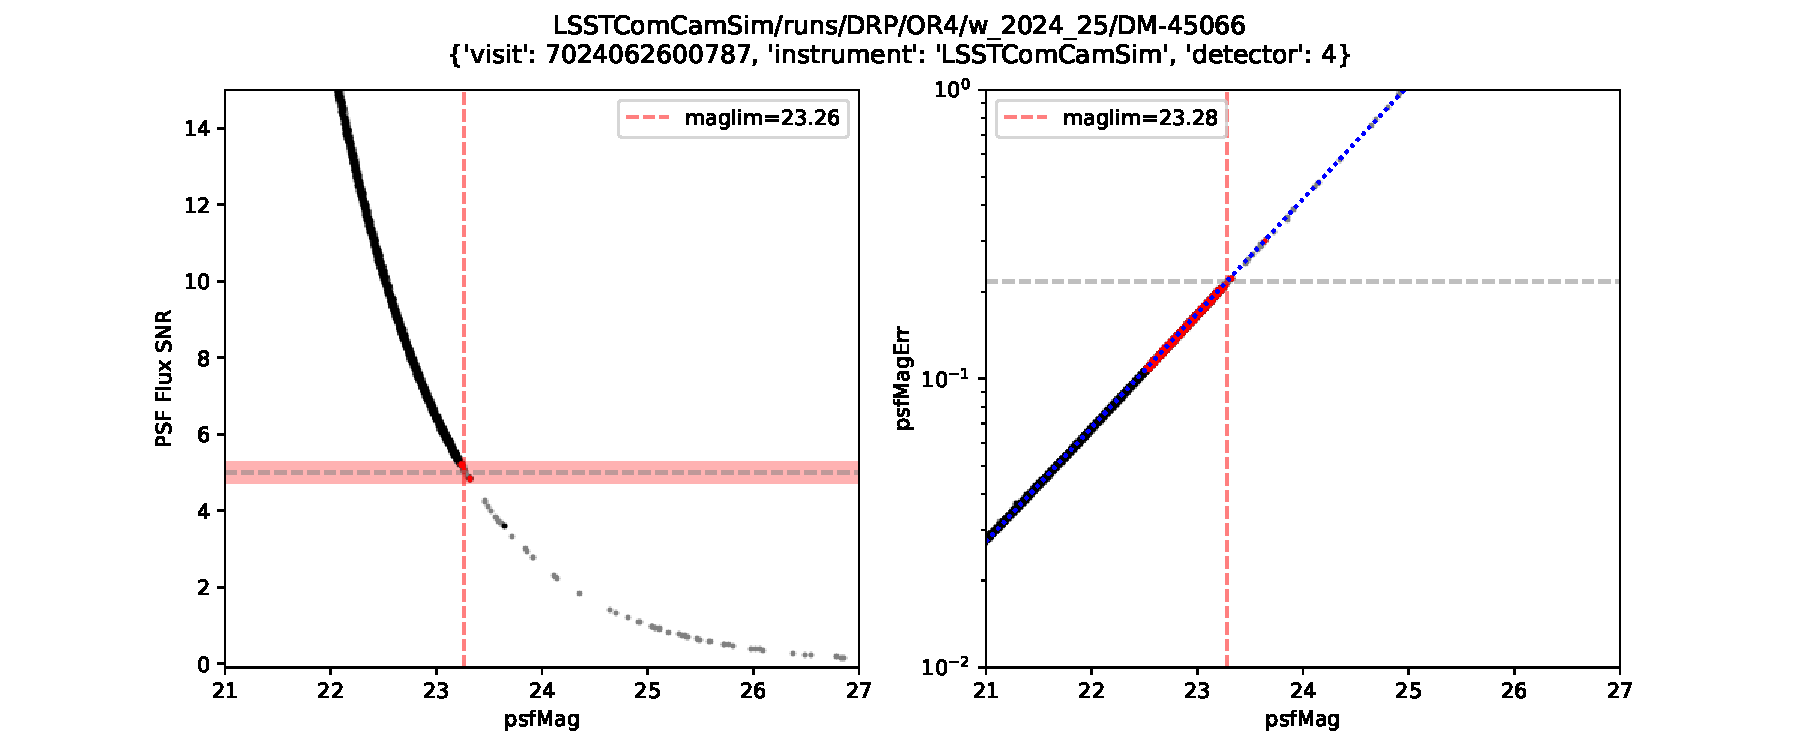
\includegraphics[width=\textwidth]{figures/or4_maglim_catalog.pdf}
    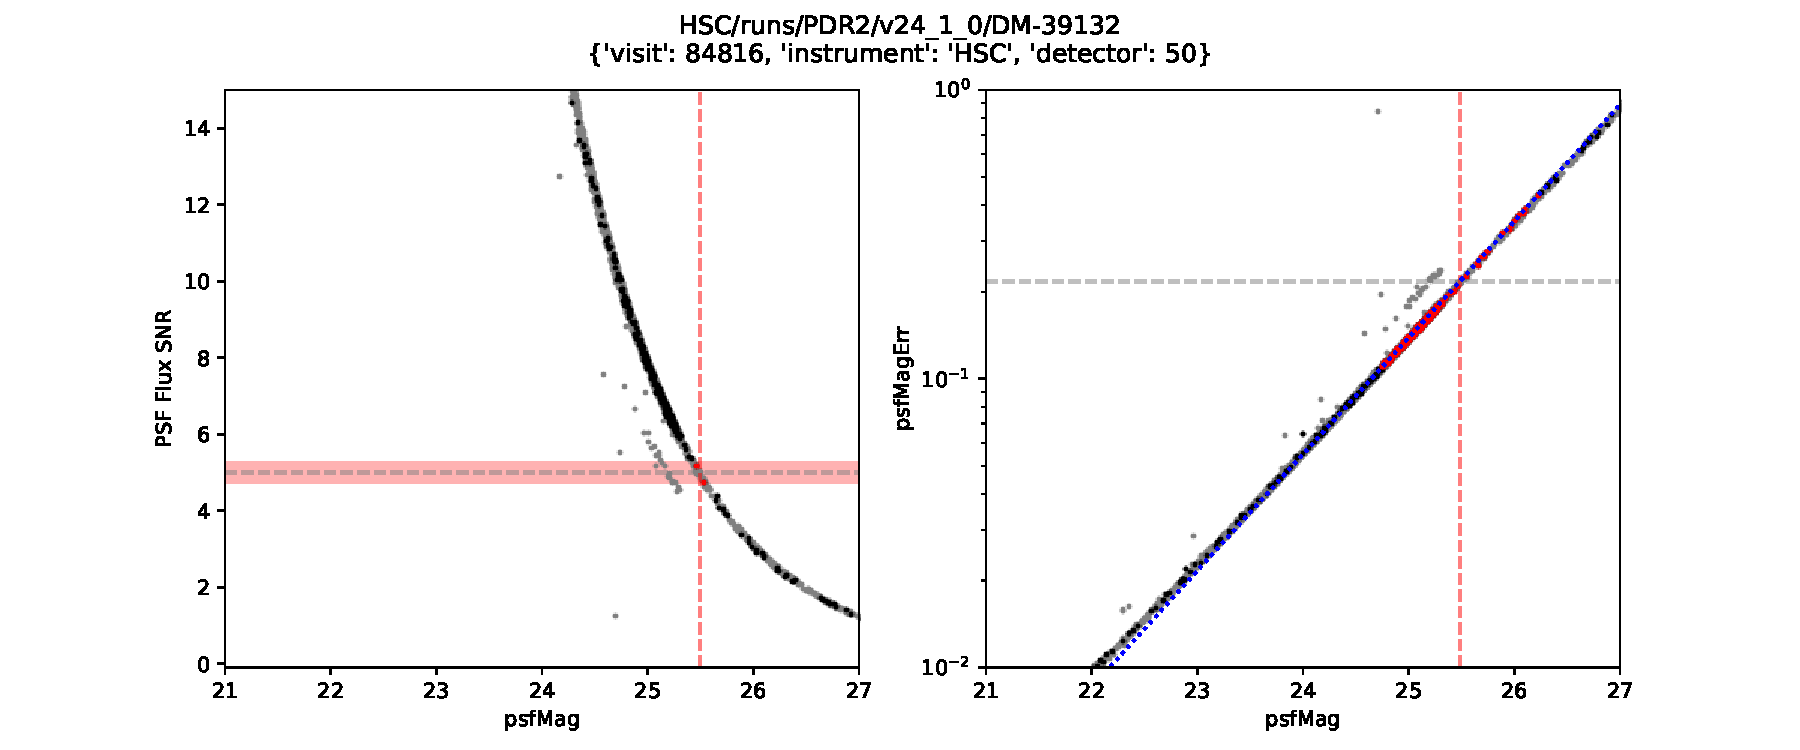
\includegraphics[width=\textwidth]{figures/hsc_pdr2_maglim_catalog.pdf}
    \caption{\label{fig:catalog} Depth estimates derived from the \texttt{psfFlux} measurements from the \texttt{SourceTable}. All sources are show in gray, while point-like sources (selected with the \texttt{extendedness} parameter) are shown in black. 
    Left panels show a SNR-based selection ($4.75 < SNR < 5.25$). Sources in this range are colored in red, while the magnitude limit is shown with the red dashed line.
    Right panels show a linear fit to the logarithm of the magnitude error vs.\ magnitude. The linear fit (blue dotted line) is performed using sources with magnitude errors close to the magnitude error threshold (red points). The linear fit is then solved for the magnitude at which magnitude error matches the desired value ($\sigma_{m5} = 0.2171$), which is shown with the red dashed line. The top panels shows results from a 30\,s simulated observation in OR4, while the bottom shows the results from a 200\,s observation from HSC PDR2.}
\end{figure*}

\section{Depth Estimates Using Exposure Summary Statistics}

A second approach to calculating the limiting magnitude of an exposure utilizes summary statistics (i.e., seeing, sky brightness, transparency, read noise). This closely follows the approach derived in \citet{LSE-40} and described in \citet{SMTN-002}. We summarize this approach and apply it to the output of the Science Pipelines for OR4.

We start by defining the relationships between image-level measurements and fluxes. The total counts from an astronomical source in an image, $C$ (ADU), can be expressed in terms of the  top-of-the-atmosphere flux, $f$ (ADU/second), atmospheric transmission coefficient $\eta$, and exposure time $t$ (seconds),\footnote{Expressed in the nomenclature of SMTN-002,
$f = \frac{1}{\eta_{\rm fid}} 10^{-\frac{2}{5}(m - ZP_{1, {\rm fid}})}$
where $m$ is the AB magnitude of the source, $ZP_{1,{\rm fid}}$ is the fiducial zeropoint for a 1-second exposure listed in the "Photometric Zeropoints" section of SMTN-002, and $\eta_{\rm fid}$ is the fiducial transmission coefficient corresponding to the "standard atmosphere" applied in that table.}
%% (This is the inverse of the flux ratio corresponding to the magnitude difference \texttt{kAtm*X} from the \texttt{syseng\_throughputs} repository?)  
\begin{align}
\label{eqn:source_counts}
C &= f \times \eta \times t.
\end{align}
The counts in an image coming from the sky, $B$ (ADU/pix), are generated from the atmosphere itself, and can be expressed in terms of the sky flux, $b$ (ADU/pix/second) and exposure time,
\begin{align}
\label{eqn:sky_counts}
B &= b \times t.
\end{align}
As described in \citet{LSE-40}, the uncertainty on the measurement of the source counts can be assembled from the variance of the total source counts, the variance of the sky background counts per pixel,\footnote{We have followed \citet{LSE-40} in ignoring the contribution of uncertainties in determining the sky background (i.e., $\sigma_B = 0$). In reality,  the determination of the mean background level can have significant uncertainty coming from spatial structure in the sky, especially at red wavelengths.} the instrumental noise per pixel, $\sigma_{\rm instr}$ (ADU/pix), and the effective number of pixels in the source footprint (i.e., the sum of pixel weights defined in Eq.~26 of \citealt{LSE-40}), $n_{\rm eff}$,
\begin{equation}
    \sigma_C^2 = C/g + (B/g + \sigma_{\rm instr}^2)  n_{\rm eff}
\end{equation}
The instrument gain, $g$ (e$^-$/ADU), enters because Poisson statistics apply to photo-electrons rather than to ADU.  For a point-like source, $n_{\rm eff}$ is equivalent to the effective area of the PSF.

The $SNR$ of a source in an image can be estimated in terms of image-level properties following \citet[][]{SMTN-002},\footnote{Eq.~\ref{eqn:snr} can be used without loss of generality if $C$, $B$, and $\sigma_{\rm instr}$ are in units of e$^-$ and $g=1$\,e$^-$/ADU.}
\begin{equation}
    \label{eqn:snr}
    SNR = \frac{C}{\sigma_C} = \frac{C}{\sqrt{C/g + (B/g + \sigma_{\rm instr}^2)  n_{\rm eff}}},
\end{equation}
From the relation between counts and flux in Eq.~\ref{eqn:source_counts} and the property of the variance of a random variate multiplied by a scalar,
\begin{align}
\label{eqn:variance}
\sigma_C^2 = \eta^2 t^2 \sigma_f^2,
\end{align}
it can be seen that
\begin{equation}
    \frac{C}{\sigma_C} = \frac{f}{\sigma_f}.
\end{equation}

Solving for the positive root of the quadratic SNR equation for $C$, it can be shown that the source counts can be expressed as,
\begin{equation}
    \label{eqn:counts}
    C(SNR, n_{\rm eff}, B, \sigma_{\rm instr}) = \frac{(SNR)^2}{2g} + \left( \frac{(SNR)^4}{4g} + (SNR)^2 \sigma_{\rm tot}^2 n_{\rm eff}  \right),
\end{equation}
where we have defined $\sigma_{\rm tot}^2 = (B/g + \sigma_{\rm instr}^2)$ to be the variance coming from background sources (i.e., the sky and instrument read noise).
The limiting magnitude can then be determined as,
\begin{equation}
    \label{eqn:stats_maglim}
    m(SNR, n_{\rm eff}, B, \sigma_{\rm instr}, ZP) = -2.5 \log_{10} \Bigl( C(SNR, n_{\rm eff}, B, \sigma_{\rm instr}) \Bigr) + ZP,
\end{equation}
where $ZP$ is the zeropoint magnitude estimated including the exposure time. Following this convention, $m5 = m(SNR=5)$ and $m10 = m(SNR=10)$. As can be seen from Eq.~\ref{eqn:counts} and \ref{eqn:stats_maglim}, the source counts and magnitude limit can be estimated assuming that we have access to the following summary measurements for an observation:
\begin{itemize}[nosep,topsep=-10pt]
    \item $B$ (\texttt{skyBg}): the sky background level [ADU or e$^-$]
    \item $n_{\rm eff}$ (\texttt{psfArea}): the effective number of pixels in the PSF [pixels]
    \item $ZP$ (\texttt{zeroPoint}): the zeropoint for the exposure [mag]\footnote{The Science Pipelines \texttt{zeroPoint} currently include the exposure time and thus $ZP = ZP_{1} + 2.5\log_{10}(t_{\rm exp})$, where $ZP_{1}$ is the zero point for a corresponding 1-second exposure and $t_{\rm exp}$ is the exposure time. There are discussions about changing \texttt{zeroPoint} to correspond to $ZP_1$ instead.}
    \item $\sigma_{\rm instr}$ (\texttt{readNoise}): the instrumental read noise [ADU or e$^-$]
    \item $g$ (\texttt{gain}): the gain (or average gain) of the detector(s) [e$^-$/ADU]
\end{itemize}

All of these parameters are available at the point of computing the exposure summary statistics. The environmental variables (i.e., \texttt{skyBg}, \texttt{zeroPoint}, and \texttt{psfArea}) are expected to vary based on observing conditions, while the other variables (i.e., \texttt{gain} and \texttt{readNoise}) are expected to be more stable from exposure-to-exposure (though this is not required). As expected, Fig.~\ref{fig:maglim} shows good agreement between the $m5$ values calculated from the exposure summary statistics and those calculated directly from the catalogs. A similar consistency check should be performed during commissioning.

\begin{figure*}[t!]
    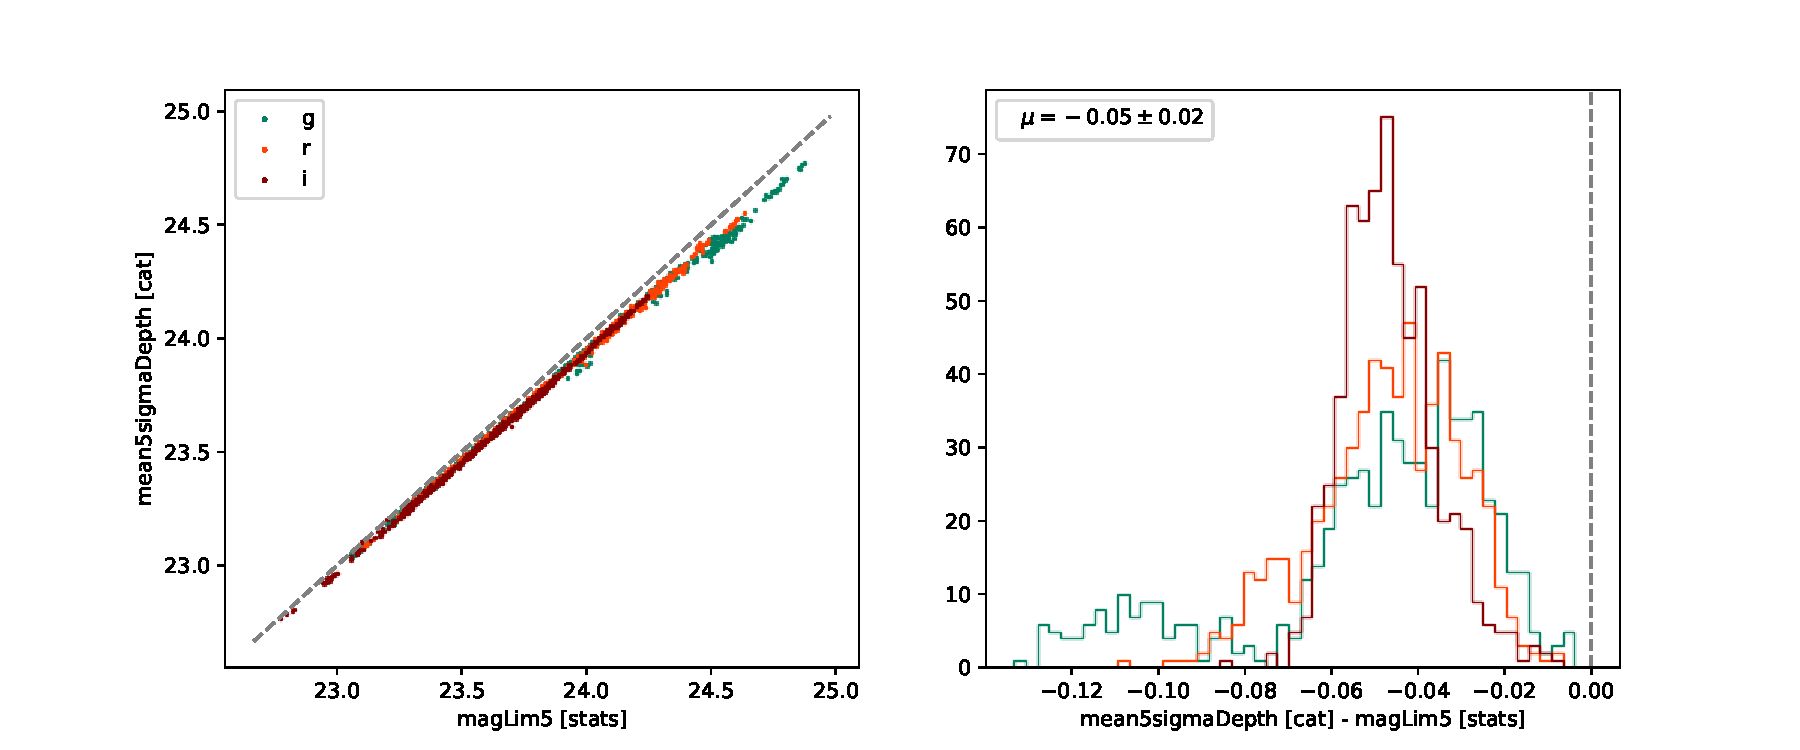
\includegraphics[width=\textwidth]{figures/or4_maglim_compare_adu_adu.pdf}
    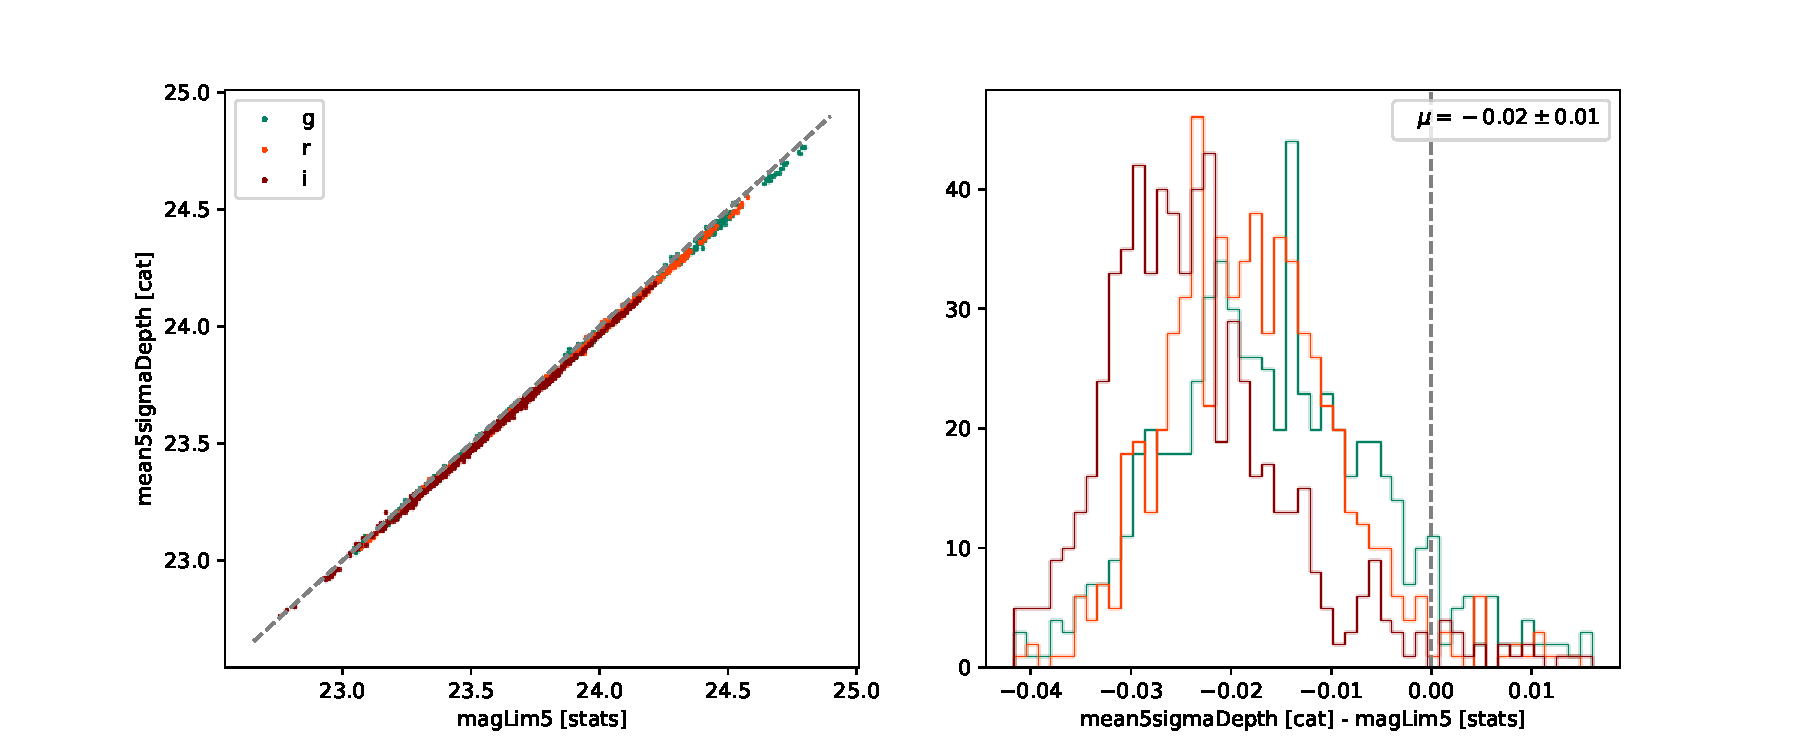
\includegraphics[width=\textwidth]{figures/or4_maglim_compare_adu_e-.pdf}
    \caption{\label{fig:maglim} Comparison between the $SNR = 5$ point-source magnitude limit for OR4 estimated from the source catalog vs.\ an estimate using exposure summary statistics. The top panel shows the comparison correctly estimating the noise variance from the image and read noise both in ADU. A deviation is seen for the deepest observations (largest magnitude limit) in the $g$ and $r$ bands. This is due to the fact that the OR4 variance plane was incorrectly calculated using the image variance in ADU and the read noise in electrons (see \href{https://rubinobs.atlassian.net/browse/DM-45976}{DM-45976}). The bottom panel uses this same (incorrect) prescription for the summary statistic depth, giving much better agreement with the catalogs.}
\end{figure*}

\section{Comparison with OpSim}
\label{sec:opsim}

\citet{SMTN-002} gives a detailed prescription for how the magnitude limit is predicted by OpSim and used for the LSST scheduler. The simulated OR4 data set gives us an opportunity to compare these predicted depth to the delivered depth estimated from the summary statistics generated with the Science Pipelines. In general, we find good agreement between the predicted depth from OpSim and the measured depth from the Science Pipelines with a scatter of $\sim 0.04$\,mag (Fig.~\ref{fig:opsim}). Furthermore, it is possible to compare the individual components going into the depth estimates (i.e., seeing, sky background, zeropoint) to see where the OpSim predictions differ from the measurements from the Science Pipelines (Appendix~\ref{app:opsim}). 

\begin{figure*}
    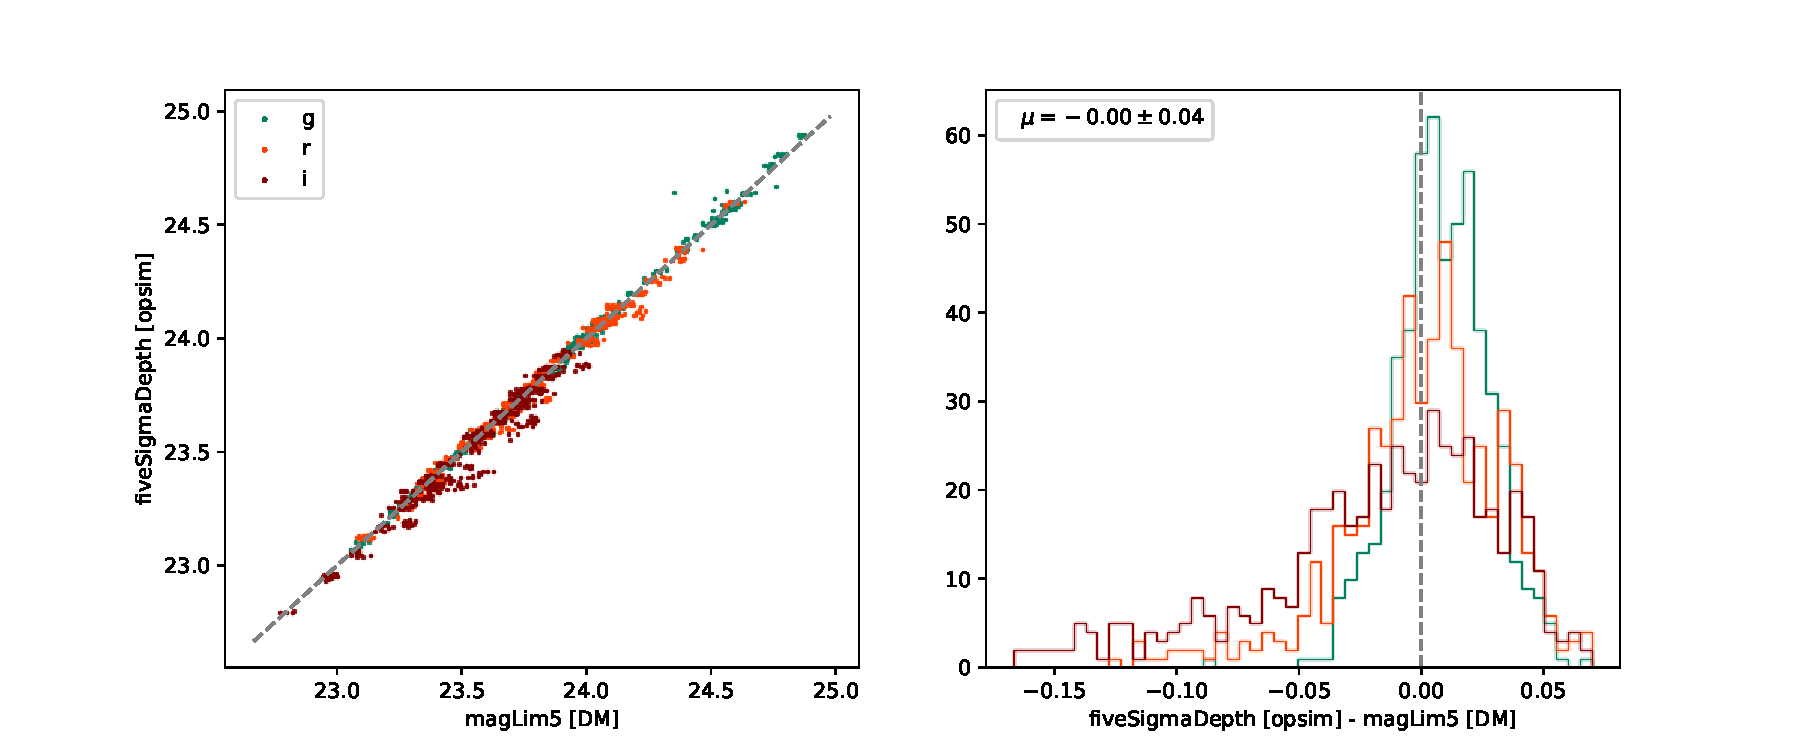
\includegraphics[width=\textwidth]{figures/or4_opsim_m5.pdf}
    \caption{\label{fig:opsim} Comparison between the $SNR=5$ point-source magnitude limit in OR4 predicted from OpSim following the prescription in \citet{SMTN-002} and the measured magnitude limit from exposure summary statistics computed by the Science Pipelines (using correct units for the image and read noise variance). The scatter between these estimates is found to be $\sim 0.04$\,mag.}
\end{figure*}

\section{Fiducial Values and Delta Magnitudes}
\label{sec:fid}

The previous discussion focused on deriving the magnitude limit for an observation without incorporating any prior knowledge about the fiducial performance of the system. However, it is often convenient to leverage fiducial values to facilitate the calculation of $m5$ (i.e., see the discussion of $C_m$ and $dC_m^{inf}$ in the final sections of \citealt{SMTN-002}) or to monitor data quality relative to some fiducial expectations of the telescope system. The fiducial depth, $m5_{\rm fid}$, can be determined from Eq.~\ref{eqn:stats_maglim} by solving 
\begin{equation}
    m5_{\rm fid} = m(SNR=5, B_{\rm fid}, n_{\rm eff,fid}, ZP_{\rm fid}, \sigma_{\rm instr,fid}).
\end{equation}
While the fiducial values can be chosen arbitrarily, we often find it most useful to define them in terms of the expected performance of the system for an observation taken at zenith in  clear, dark condition with the characteristic atmospheric seeing. These fiducial values can be set in a number of ways --- in the context of Rubin, they can be taken from the SRD, from the current best estimates of the expected system performance \citep{SMTN-002}, or from actual observations during nominal conditions. However, it is important to minimize the redefinition of fiducials in order to preserve the relative differences between the observed data and the fiducials.

We refer to the difference between the depth of an observation, $m5$, and the fiducial depth, $m5_{\rm fid}$, as the ``delta magnitude'', 
\begin{equation}
    \Delta m5 =  m5 - m5_{\rm fid}.
\end{equation}
If the fiducial values are set based on the nominal conditions, then $\Delta m5$ will generally be negative, though this need not always be the case. Furthermore, the impact  of each individual observational component (i.e., seeing, sky background, transparency, read noise) can be assessed independently by calculating the delta magnitude holding all other components fixed at their fiducial values. For example, the importance of the sky can be isolated by calculating
$\Delta m5_{\rm sky} = m5_{\rm sky} - m5_{\rm fid}$,
where we define $m5_{\rm sky} = m(SNR=5, B, n_{\rm eff,fid}, ZP_{\rm fid}, \sigma_{\rm instr,fid})$ to be the depth estimated fixing all components at their fiducial values except the measured sky background.


\section{Coadded depth and effective number of exposures}
\label{sec:coadd_depth}


The $m5$ depth of a coadded image can be easily computed from the depth of individual images assuming that the uncertainty on the (top-of-the-atmosphere) flux of a source, $f$, is uncorrelated between the individual images that contribute to the coadd. In this case, we can use the standard formula for propagation of errors in an inverse-variance-weighted mean to get the coadd uncertainty,
\begin{equation}
\label{eqn:ivwpoe}
\sigma_{f,\rm{coadd}}^{-2} = \sum_i \sigma_{f,i}^{-2}.
\end{equation}
This formula holds when $\sigma_{f,i}$ is the standard deviation in the top-of-the-atmosphere flux, $f$, for input image $i$.
In this situation, the flux is independent of exposure time, and Eq.~\ref{eqn:ivwpoe} makes it clear that two exposures of different exposure times but the same uncertainty ($\sigma_{f,i} = \sigma_{f,j}$) will have the same contribution to the coadded flux uncertainty, $\sigma_{f, {\rm coadd}}$.

Transforming our equation for the limiting magnitude (Eq.~\ref{eqn:stats_maglim}) from counts in the image, $C$, to flux, $f$,
\begin{align}
m(SNR) &= -2.5 \log_{10}(C) + ZP \\
       &= -2.5 \log_{10}(f) - 2.5\log_{10}(\eta \times t) + ZP \\
       &= -\frac{5}{2} \log_{10}({SNR} \times \sigma_f) + m_0,
\end{align}
where $t$ is the exposure time, $\eta$ is the atmospheric transmission (fraction of photons that make it through the atmosphere), and in the last line we have defined a scaled zero point that is independent of exposure time and extinction (i.e., the zero point for an exposure time of 1\,s and no atmosphere), $m_0 = ZP - 2.5\log_{10}(\eta \times t)$.
%This relationship For both the coadd and individual exposures the flux corresponding to $m_{SNR}$ is ${\rm SNR} \times \sigma_{F}$, such that
Working with the scaled zero point $m_0$ is convenient so the same value can be used for both the coadd and all of the contributing exposures, independent of exposure time. 
Re-arranging, we get
\begin{align}
\sigma_f &= \frac{1}{{SNR}} 10^{-\frac{2}{5} (m_{SNR} - m_0)}.
\end{align}
If we substitute $\sigma_f$ above into the propagation of errors formula (Eq.~\ref{eqn:ivwpoe}) and solve for $m_{SNR}$, we get,
\begin{equation}
m_{SNR,{\rm coadd}} = \frac{5}{4} \log_{10}\Bigl( \sum_i 10^{\frac{4}{5}m_{{SNR}, i}} \Bigr).
\end{equation}
Note that both $SNR$ and $m_0$ cancel out completely; the above formula is independent of the magnitude zero point and applies to any $SNR$.

This relationship between the coadd depth and the depth of contributing exposures is not linear, and common questions regarding depth are difficult to intuit from $m5$ alone without resorting to using a computer. For example, given the depth of a coadd, it is difficult to intuit what fraction of progress has been made toward a target depth, or how much an additional exposure with a known $m5$ will improve the coadd depth. Such estimates are easier to intuit with a linear measure of progress.

Inspection of the propagation of errors equation (Eq.~\ref{eqn:ivwpoe}) indicates that there is such a linear metric, $\sigma_f^{-2}$. Its scaling and units (inverse flux squared) are not particularly intuitive; however, as a linear quantity, we can scale it to something more convenient. Let us define a new value, $\tau$, that is $\sigma_f^{-2}$ scaled such that an exposure with a nominal exposure time taken under fiducial conditions has $\tau=1$. In this case, $\tau$ for a given exposure represents its contribution to the $SNR$ of a coadd relative to a nominal exposure, and $\tau$ for a coadd represents the number of nominal exposures that would need to be coadded to achieve the same $m5$:
\begin{align}
\tau &= \sigma_{f, {\rm nom}}^2 \sigma_f^{-2} \\
\sigma_f &= \sigma_{f, {\rm nom}} \tau^{-\frac{1}{2}}
\end{align}
Substituting $\tau$ in place of $\sigma_f$ in the equations for $m_{\rm SNR}$ as a function of $\sigma_f$ and its inverse:
\begin{align}
m_{\rm SNR} &= \frac{5}{4} \log_{10}(\tau) + m_{\rm SNR,nom} \\
\tau &= 10^{\frac{4}{5} (m_{\rm SNR} - m_{\rm SNR,nom})},
\end{align}
where $m_{SNR, {\rm nom}}$ is the nominal magnitude limit at a given $SNR$---i.e.,  $m_{SNR, {\rm fid}}$ evaluated for the nominal WFD exposure time (e.g., $t_{\rm WFD} = 30$\,s). So, for the standard $SNR = 5$:
\begin{align}
\tau  &= 10^{\frac{4}{5} (m5 - m5_{\rm nom})} \\
m5 &= \frac{5}{4} \log_{10}(\tau) + m5_{\rm nom} \\
\tau_{\rm coadd} &= \sum_i \tau_i.
\end{align}

Conceptually, $\tau_{\rm coadd}$ for a coadd (including a coadd of just one exposure) is the number of nominal WFD exposures (i.e., exposures taken in fiducial conditions and instrument sensitivity and nominal WFD exposure time) that it would take to achieve the same $m5$ as that coadd. So, one can think of the accumulated $\tau$ of a coadd as a number to compare with the accumulated number of exposures in order to take data quality into account.

\section{Effective Exposure Time}
\label{sec:teff}

An alternative interpretation of the linear metric, $\sigma_f^{-2}$, is as an effective exposure time \citep{Neilsen:2016}. Starting from the expression for SNR in terms of the image counts (Eq.~\ref{eqn:snr}) and converting to fluxes (Eq.~\ref{eqn:source_counts} and \ref{eqn:sky_counts}), we can express the SNR in terms of the flux as,
\begin{align}
{\rm SNR} = \frac{C}{\sigma_C} &= \frac{f \eta t}{\sqrt{\frac{f \eta t}{g} + \frac{b t}{g}n_{\rm eff} + \sigma_{\rm inst}^2 n_{\rm eff}}} \\
& = f \times \sqrt{ \frac{\eta^2 t^2}{\frac{f \eta t}{g} + \frac{b t}{g}n_{\rm eff} + \sigma_{\rm inst}^2 n_{\rm eff}}} \\
& = f \times \sqrt{ \frac{\eta^2 t^2}{\sigma_C^2} } = \frac{f}{\sigma_f}.
\end{align}
%& = f \times \sqrt{ \frac{g \eta^2}{f \eta + b n_{\rm eff} + \frac{g}{t} \sigma_{\rm inst}^2 n_{\rm eff}} \times t}  
Rearranging a bit, we find
\begin{equation}
\sigma_f^{-2} = \left[ \frac{g \eta^2}{f \eta + b n_{\rm eff} + \frac{g}{t}\sigma_{\rm inst}^2 n_{\rm eff}}  \right] \times t .
\end{equation}

If we are in the regime where the sky background dominates, then the middle term in the denominator dominates over the others, and we are left with
\begin{equation}
\label{eqn:skydomsnr}
    {\rm SNR} \approx f \times \sqrt{ \frac{g \eta^2}{ b n_{\rm eff}}  \times t }.
\end{equation}
DES {\it aficionados} will recognize Eq.~\ref{eqn:skydomsnr} as the starting point for defining the effective exposure time, $t_{\rm eff}$, as described in \citet{Neilsen:2016}.
So long as $\sigma_{\rm inst}$ is small (i.e., the noise is dominated by the Poisson shot-noise from the source and sky), then $\sigma_f^{-2}$ is proportional to the exposure time.
This gives another way to scale $\sigma_f^{-2}$ to make it more intuitive: a hypothetical equivalent exposure time under fiducial conditions assuming that there is only noise from Poisson statistics. 

If we define $t_{\rm eff}$ to be another scaling of $\sigma_f^{-2}$ such that:
\begin{equation}
t_{\rm eff} = \sigma_{f, {\rm nom}}^2 \sigma_f^{-2} \times t_{\rm WFD} = \tau \times t_{\rm WFD} 
\end{equation}
where $t_{\rm WFD}$ is the nominal WFD exposure time, then $t_{\rm eff}$ will be approximately equal to the exposure time it would take to get an exposure of equivalent $m5$ depth, where the approximation ``breaks down'' when $\sigma_{\rm inst}^2$ is significant.
Following the discussion in Section~\ref{sec:coadd_depth}, the relation between $t_{\rm eff}$ and $m5$ is,
\begin{align}
t_{\rm eff} &= 10^{\frac{4}{5} (m5 - m5_{\rm nom})} \times t_{\rm WFD}  \\
m5 &= \frac{5}{4} \log_{10}(t_{\rm eff}) - \frac{5}{4} \log_{10}(t_{\rm WFD}) + m5_{\rm nom} \\
t_{\rm eff, coadd} &= \sum_i t_{{\rm eff},i}.
\end{align}
These relations between $t_{\rm eff}$ and $m5$ hold even when $\sigma_{\rm inst}$ is significant: a significant $\sigma_{\rm inst}$ only breaks the metaphor with exposure time, not the relationship between a scaled $\sigma_f^{-2}$ and limiting magnitude.

\section{Summary}
\label{sec:summary}
Measuring the depth of astronomical observations is important for the purposes of modeling system performance, estimating survey progress, and selecting subsets of exposures for further downstream processing. The depth can be calculated independently of any fiducial system performance values (assuming that a zero point can be determined); however, the comparison against fiducial values provides convenient metrics for monitoring operational performance. In this note, we have described the calculation of the limiting $5\sigma$ point-source magnitude, $m5$, from source catalogs and exposure summary level statistics. The two provide a useful crosscheck, and show good agreement in the OR4 simulated data (once known issues are accounted for). However, this agreement is expected since the flux uncertainties in the source catalog come from the same variance calculation as is used in the summary statistic calculation. Another useful independent assessment of the depth and photometric uncertainties will come from repeated measurements of faint (and/or sky) sources. While more difficult to implement, such a check is important to validate the analytic variance calculation.

\appendix

\section{OpSim Comparison}
\label{app:opsim}

This appendix shows comparisons between the seeing, sky brightness, and zeropoints predicted from OpSim vs.\ those estimated from the Science Pipelines using the central detector (\texttt{detector=4}) of OR4. It is necessary to do some translations to convert from the native OpSim parameters and DM measurements, which we describe below:
\begin{itemize}
    \item ${\rm psfArea}_{\rm opsim} = 2.266 \times ({\rm seeingFwhmEff}/{\rm pixscale})^2$
    \item ${\rm skyBg}_{\rm opsim} = {\rm skycounts}/{\rm gain}$
    \item ${\rm zeroPoint}_{\rm opsim} = {\rm zeropoint} + 2.5 \log_{10}({\rm expTime}) - 2.5\log_{10}({\rm gain})$
\end{itemize}
where \texttt{seeingFwhmEff}, \texttt{zeropoint}, and \texttt{skycounts} are native quantities provided by OpSim, and ${\rm gain} \approx 1.67$\,e$^-$/ADU, ${\rm pixscale} = 0.2$\,arcsec/pix, and ${\rm expTime} = 30$\,seconds for OR4. Once these translations are performed, we find that the OpSim predictions and the DM measurements agree to within $\lesssim10\%$. The sky brightness predicted by OpSim is found to be $\sim 7\%$ smaller (fainter) than that measured by DM with a clear trend from bluer to redder bands. Similarly, the \texttt{zeroPoint} predicted by OpSim is smaller (shallower) by $\sim 0.05$\,mag ($\sim 0.05\%$) relative to the measured value from DM. 

\begin{figure*}
    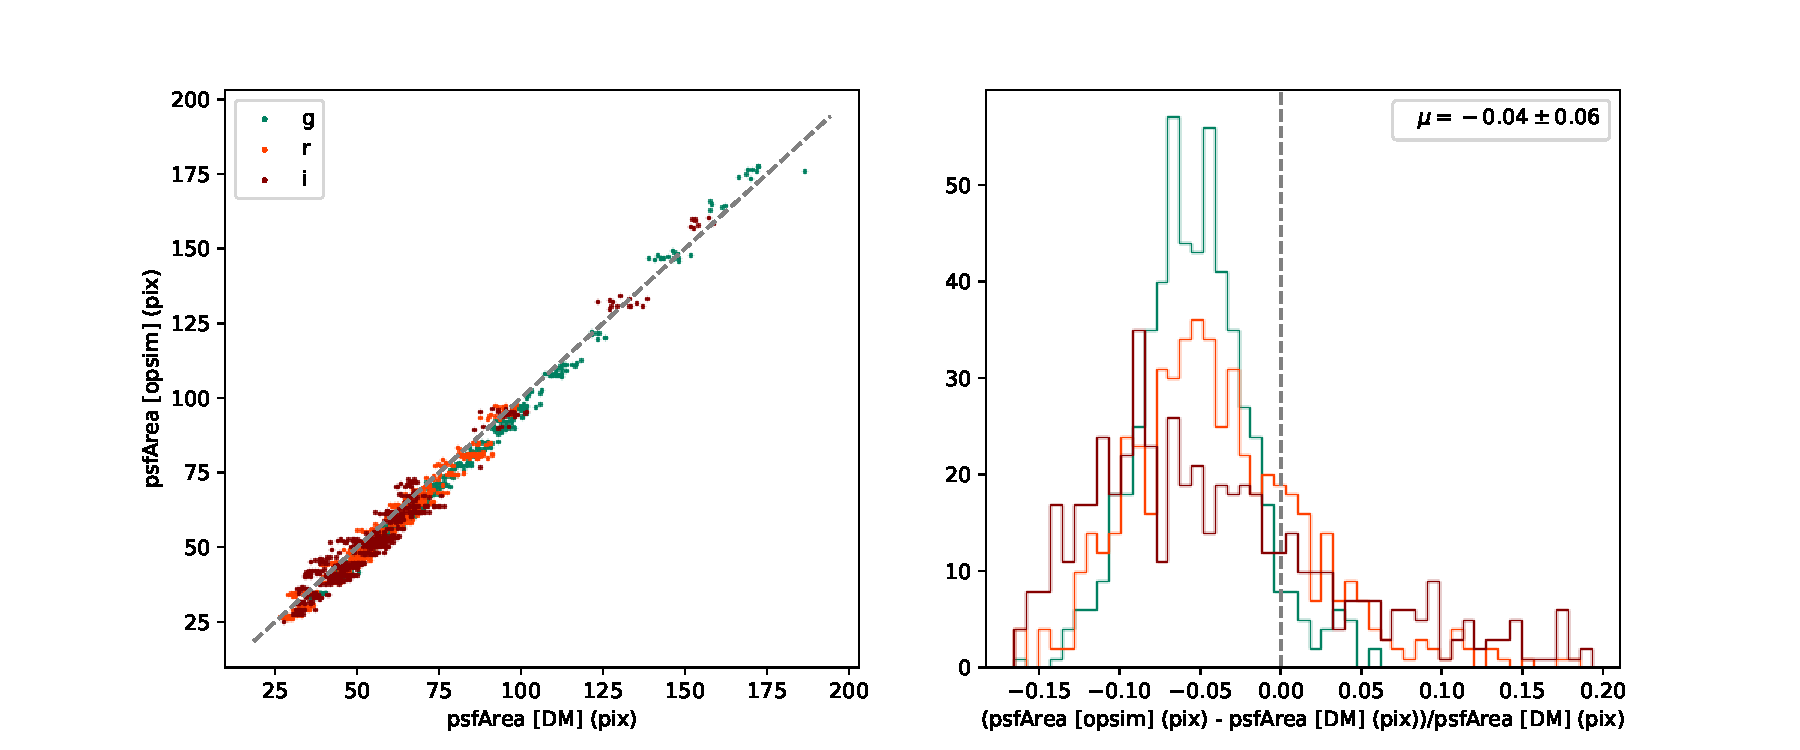
\includegraphics[width=\textwidth]{figures/or4_opsim_psf.pdf}
    \caption{\label{fig:opsim_psf} Comparison between the effective size of the PSF (in pixels) predicted by OpSim and that measured by DM.}
\end{figure*}

\begin{figure*}
    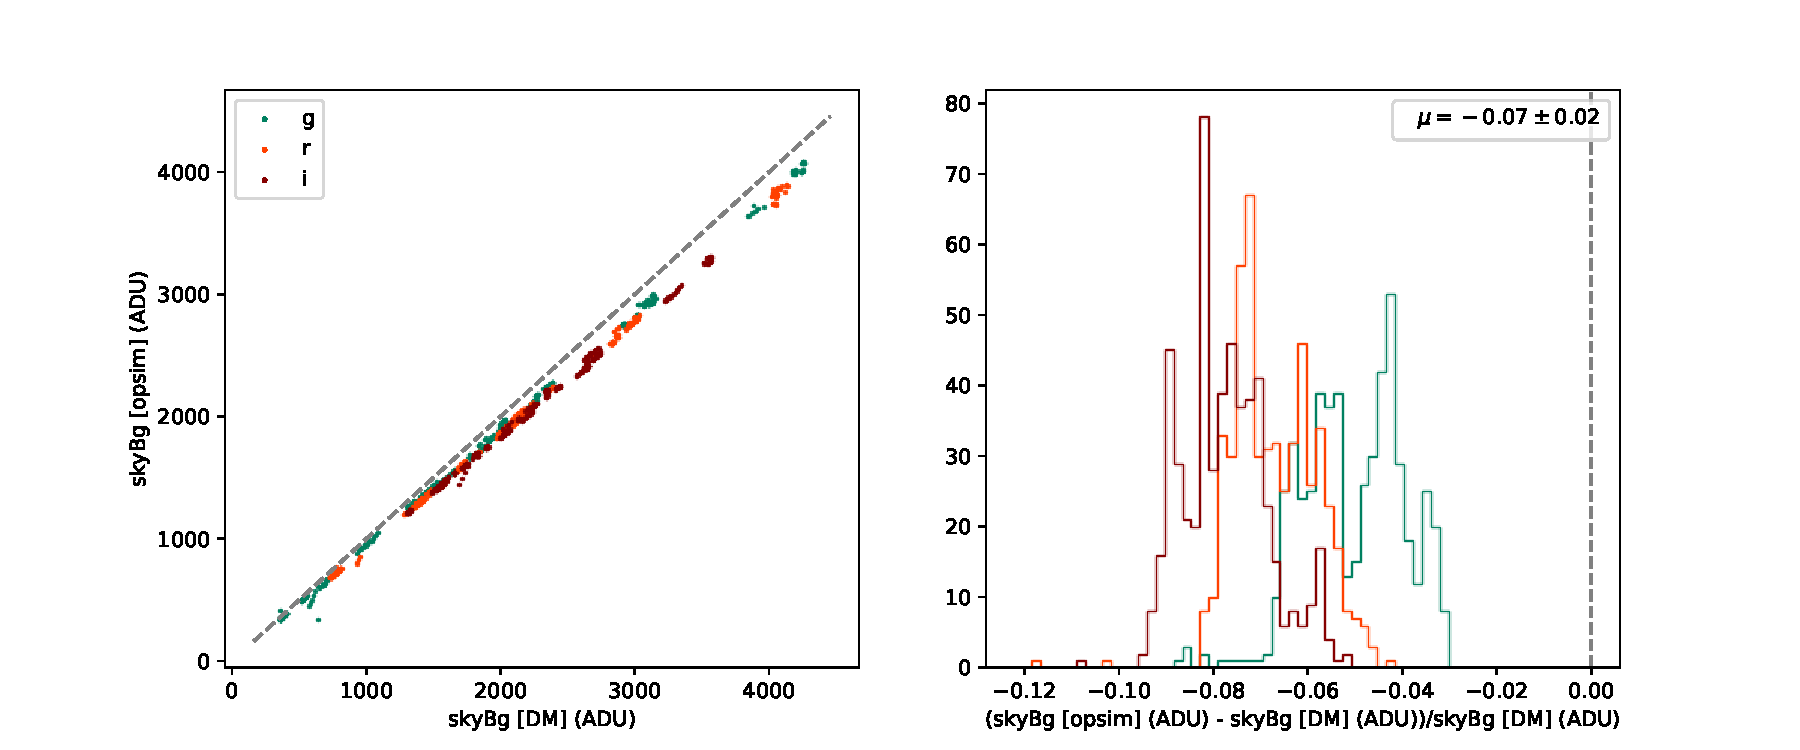
\includegraphics[width=\textwidth]{figures/or4_opsim_sky.pdf}
    \caption{\label{fig:opsim_sky} Comparison between the sky background (in ADU) predicted by OpSim and that measured by DM.}
\end{figure*}

\begin{figure*}
    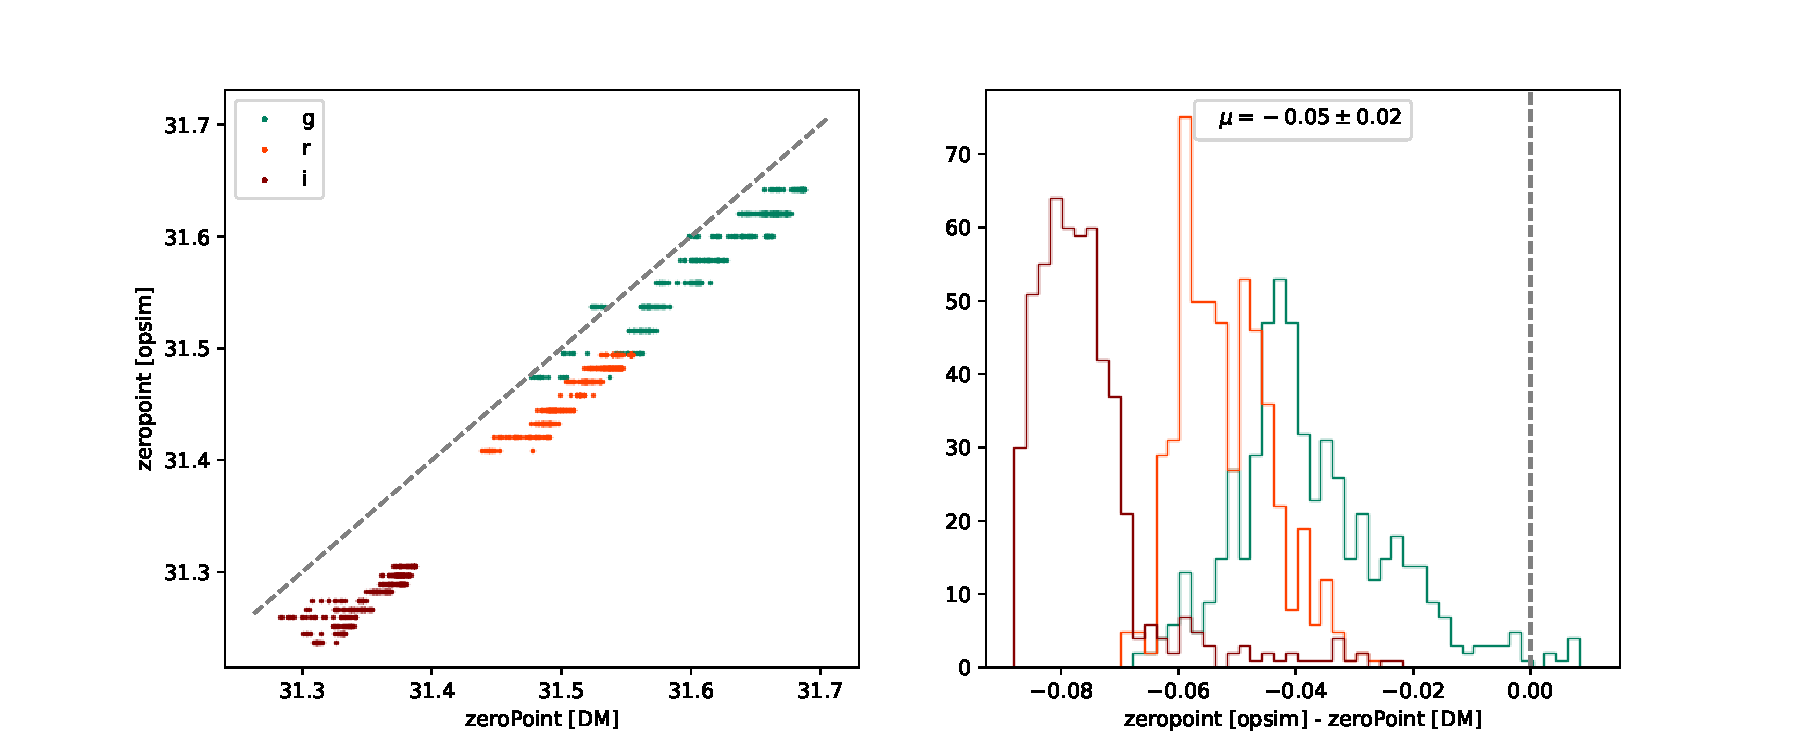
\includegraphics[width=\textwidth]{figures/or4_opsim_zeropoint.pdf}
    \caption{\label{fig:opsim_zp} Comparison between the zero point (in ADU and including the exposure time) predicted by OpSim and that measured by DM.}
\end{figure*}

\clearpage

% Include all the relevant bib files.
% https://lsst-texmf.lsst.io/lsstdoc.html#bibliographies
\section{References} \label{sec:bib}
\renewcommand{\refname}{} % Suppress default Bibliography section
\bibliography{local,lsst,lsst-dm,refs_ads,refs,books}

% Make sure lsst-texmf/bin/generateAcronyms.py is in your path
\section{Acronyms} \label{sec:acronyms}
\addtocounter{table}{-1}
\begin{longtable}{p{0.145\textwidth}p{0.8\textwidth}}\hline
\textbf{Acronym} & \textbf{Description}  \\\hline

ADU & Analogue-to-Digital Unit \\\hline
B & Byte (8 bit) \\\hline
DES & Dark Energy Survey \\\hline
DM & Data Management \\\hline
DMTN & DM Technical Note \\\hline
DR2 & Data Release 2 \\\hline
HSC & Hyper Suprime-Cam \\\hline
LSE & LSST Systems Engineering (Document Handle) \\\hline
LSR & LSST System Requirements; LSE-29 \\\hline
LSS & Large Scale Structure \\\hline
LSST & Legacy Survey of Space and Time (formerly Large Synoptic Survey Telescope) \\\hline
OpSim & Operations Simulation \\\hline
PDR2 & Public Data Release 2 (HSC) \\\hline
PSF & Point Spread Function \\\hline
SNR & Signal to Noise Ratio \\\hline
SRD & LSST Science Requirements; LPM-17 \\\hline
WFD & Wide Fast Deep \\\hline
\end{longtable}

% If you want glossary uncomment below -- comment out the two lines above
%\printglossaries

\end{document}

\begin{comment}
\section{Flux Variance Derivation}

In Section~\ref{sec:teff} we derived the flux variance from the SNR. However, it may be useful to see how the flux variance can be derived directly from the variance on the counts. The top of the atmosphere count rate (ADU/second), $f$, is derived from the electrons counted in the image from the object, $e$, in the exposure time, $t$ (seconds), corrected by the atmospheric transmission coefficient $\eta$ and gain, $g$ (e-/ADU),
\begin{equation}
f = \frac{e}{t \times \eta \times g}
\end{equation}
The variance in the flux is therefore,
\begin{equation}
\label{eqn:vare}
\sigma_f^2 = \frac{ \sigma_{e}^{2} }{ t^2 \eta^2 g^2 }.
\end{equation}

The variance corresponding to the uncertainty in our estimate of electrons counted from the object has three major statistical components: 
(1) variance from the Poisson noise in electrons counted from the object itself,
\begin{equation}
\sigma_{e, \texttt{object}}^2 = f \times t \times g  \times \eta ,
\end{equation}
(2) the variance from the sky background,
\begin{equation}
\sigma_{e, \texttt{sky}}^2 = b \times t \times g \times n_{\texttt{eff}},
\end{equation}
and (3) the variance from the read noise,
\begin{equation}
\sigma_{e, \texttt{rn}}^2 = (\sigma_{\texttt{inst}} \times g)^2 \times n_{\texttt{eff}}.
\end{equation}
Combining the sources of variance, we get:
\begin{align}
\sigma_{e}^{2} & = \sigma_{e, \texttt{object}}^2 + \sigma_{e, \texttt{sky}}^2 + \sigma_{e, \texttt{rn}}^2 \\
& = f t g \eta
+ b t g n_{\texttt{eff}}
+ (\sigma_{\texttt{inst}}  g)^2 n_{\texttt{eff}}
\end{align}
Substituting the expression for $\sigma_{e}^{2}$ in Eq.~\ref{eqn:vare} and solving for $\sigma_f^{-2}$, we get,
\begin{equation}
\label{eqn:varf}
\sigma_f^{-2} = \left[ \frac{g \eta^2}{f \eta + b n_{\rm eff} + \frac{g}{t}\sigma_{\rm inst}^2 n_{\rm eff}}  \right] \times t .
\end{equation}

If $\sigma_{\rm inst}$ is small such that the uncertainty is dominated by the Poisson noise from the source and sky, then $\sigma_f^{-2}$ is proportional to the exposure time, and we have a second way of scaling $\sigma_f^{-2}$ to make it comparable to something meaningful: a hypothetical equivalent exposure time under fiducial conditions assuming that there is only noise from Poisson statistics.
If we define $t_{\rm eff}$ to be another scaling of $\sigma_f^{-2}$ such that:
\begin{equation}
t_{\rm eff} = \tau \times t_{\rm WFD} 
\end{equation}
where $t_{\rm WFD}$ is the nominal WFD exposure time, then $t_{\rm eff}$ will be approximately equal to the exposure time it would take to get an exposure of equivalent $m5$ depth, where the approximation ``breaks down'' when $\sigma_{\rm inst}^2$ is significant.\footnote{
If we are in the domain where the sky background dominates, then the middle term in the denominator in Eq.~\ref{eqn:varf} dominates over the others. If we derive a signal to noise ratio ($\texttt{SNR}$) from the result, we are left with
\begin{equation}
\label{eqn:skydomsnrv1}
    {\rm SNR} = \frac{f}{\sigma_{f}} = f \times \sqrt{ \frac{g \eta^2}{ b n_{\rm eff}}  \times t }.
\end{equation}
DES {\it aficionados} should recognize this as the scaling for the effective exposure time, $t_{\rm eff}$, as used in DES, with Eq.~\ref{eqn:skydomsnrv1} corresponding to Eq.~1 of \cite{Neilsen:2016}: the use of $t_{\rm eff}$ in this note is a generalization of its use in DES, adding terms to account for uncertainty due to object Poisson noise and read noise, both of which were negligible near the limiting magnitude of DES images.
}


The relation between $t_{\rm eff}$ and $m5$ is then:
\begin{align}
t_{\rm eff} &= t_{\rm WFD} \times 10^{\frac{4}{5} (m5 - m5_{\rm nom})} \\
m5 &= \frac{5}{4} \log_{10}(t_{\rm eff}) - \frac{5}{4} \log_{10}(t_{\rm WFD}) + m5_{\rm nom} \\
t_{\rm eff, coadd} &= \sum_i t_{{\rm eff},i}
\end{align}

These relations between $t_{\rm eff}$ and $m5$ hold even for exposures for which $\sigma_{\rm inst}$ is significant: a significant $\sigma_{\rm inst}$ only breaks the metaphor with exposure time, not the relationship between a scaled $\sigma_F^{-2}$ and limiting magnitude.
\end{comment}
